\section{Technical Background}

Before any progress on the topic can be made, however, we need to overcome some technical hurdles, which, regarding the main research question of this thesis might not seem important, but they are in their own way essential.

Furthermore, in this section we will discuss some of the technical aspects of this thesis, such as different types of RGB-D cameras and how they work. Since multiple cameras are used we will also discuss if they work together or if there is interference.

Firstly, we will focus on RGB-D Cameras and how they work together and in the program that was developed in the scope of this thesis. Afterwards, we discuss the visual representation of the point-cloud. Finally, we will focus on the mathematical theory behind synchronising multiple cameras. 

\subsection{RGB-D Cameras}

RGB-D Cameras or depth cameras offer, as the name suggests an RGB feed of a scene as well as the depth of every pixel. Such an image can be recorded using several different methods. Most cameras however work with infrared light.

\subsubsection{Structured Light Cameras}

\subsubsection{Time of Flight Cameras}

\subsubsection{Machine Learning Approach}

In addition to hardware approached for depth detection there are also Software solutions to determine the depth corresponding to a specific pixel in an image. Examples for this kind of depth estimation is for example monocular depth estimation \cite{mono_depthestimation_bts, mono_depthestimation_depthformer, mono_depthestimation_glpn}, which uses a single image to estimate the depth, and multi-view or stereo depth estimation \cite{multiview_depthestimation_epipolar, multiview_depthestimation_fusion, multiview_depthestimation_RealSense_and_any}, which as the name suggests utilises multiple view angles to estimate the depth of a scene.

While these methods are interesting they will not be focused on in this thesis, since most are not yet applicable in real-time applications due to slow estimation time.

\subsection{Tuning RGB-D cameras}

The depth measurement relies on Infrared emitters and respective sensors. The sensors and emitters can be tweaked for a specific scene. 
refer to \hyperlink{https://dev.intelrealsense.com/docs/tuning-depth-cameras-for-best-performance}{"Tuning depth cameras for best performance"} for more information.

\subsection{Reading Data of RGB-D cameras}

To read depth images we poll a depth frame. This depth then needs to be transformed into the same space as the other cameras. To understand how this can be done we need to understand the way depth images are created. In figure (create figure) we can see a standard depth image of an indoor scene. The depth of each pixel is denoted with grey tone corresponding with a specific depth. 

This 2 dimensional pixel representation cannot be directly translated into the 3d camera coordinate system, this process is called \textit{Camera Calibration}. In \cite{camera_calibration} Z.Zhang introduced a method that utilises the intrinsics of a specific camera in a 3x3 matrix. This intrinsic matrix contains the principle point $(c_0, c_0)$ the scale factor or focal length $f_x$ and $f_y$. In this thesis we use the pinhole camera model and don't account for distortion. The setup using a simplified pinhole camera can be seen in Figure \ref{fig:pinhole}.

\begin{figure}[h]
    \centering
    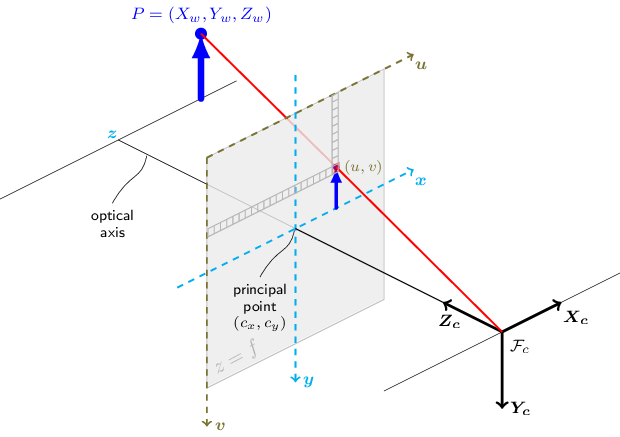
\includegraphics[width=.9\linewidth]{figures/CameraCalibration/pinhole_camera_model.png}
    \caption{Pinhole Camera Model}
    \label{fig:pinhole}
\end{figure}

Using this we can calculate the world position $P = (X_w, Y_w, Z_w)$ given the camera coordinates $(u, v)$ and the focal-length using equation \ref{eq}.


\subsection{Synchronisation of multiple RGB-D cameras}

To synchronise the coordinate system of each camera we first need to reduce the degree of freedom of each camera in their individual camera space. For this we assume that the cameras both view the same floor, if this is not a given then synchronisation with this method will be very hard.

The synchronisation process goes as follows:

RGBD -> Camera Space -> Joined World Space

Once the cameras are adjusted and have the same distances we can find a way to overlay the pointclouds

\subsubsection{Floor detection}

After the depth stream has been properly back projected into 3D world space we detect the floor. This is done using random sampling consensus (RANSAC). We select 3 points at random and create a plane. Then we count the points that are within a certain threshold of that plane and take note. We do this for several iterations until we have found the largest plane. This approach is used in countless other applications which aim to do plane segmentation in point clouds. \cite{floor-detection}.
